\section{Introduction}
\label{sec:intro}

Autonomous navigation in complex environments is a critical capability for robots operating in various applications, such as military reconnaissance ~\cite{reconn1}, search and rescue missions ~\cite{sar1}, and surveillance operations ~\cite{surv1}. These scenarios pose unique challenges for robots, requiring them to accurately perceive the environment, identify potential cover, and adapt their navigation strategies to minimize exposure to threats while efficiently reaching the goal. In this context, a threat is any external factor capable of recognizing or interfering with the agent's presence and objectives. Developing robust navigation strategies that can effectively navigate in these environments while maintaining covertness is a challenging task, as it requires accounting for various uncertainties, dynamic obstacles, and environmental factors. Existing approaches to covert navigation often rely on pre-defined environmental models ~\cite{predef1, predef2} or supervised learning techniques ~\cite{sup1, sup2} that require extensive manual annotation and labeling of traversable terrain. However, these methods may not align with the actual traversability capabilities of different robots due to varying dynamic constraints, leading to conservative and inefficient navigation behaviors ~\cite{conserv1, conserv2}.

\begin{figure}[!htb]
    \centering
    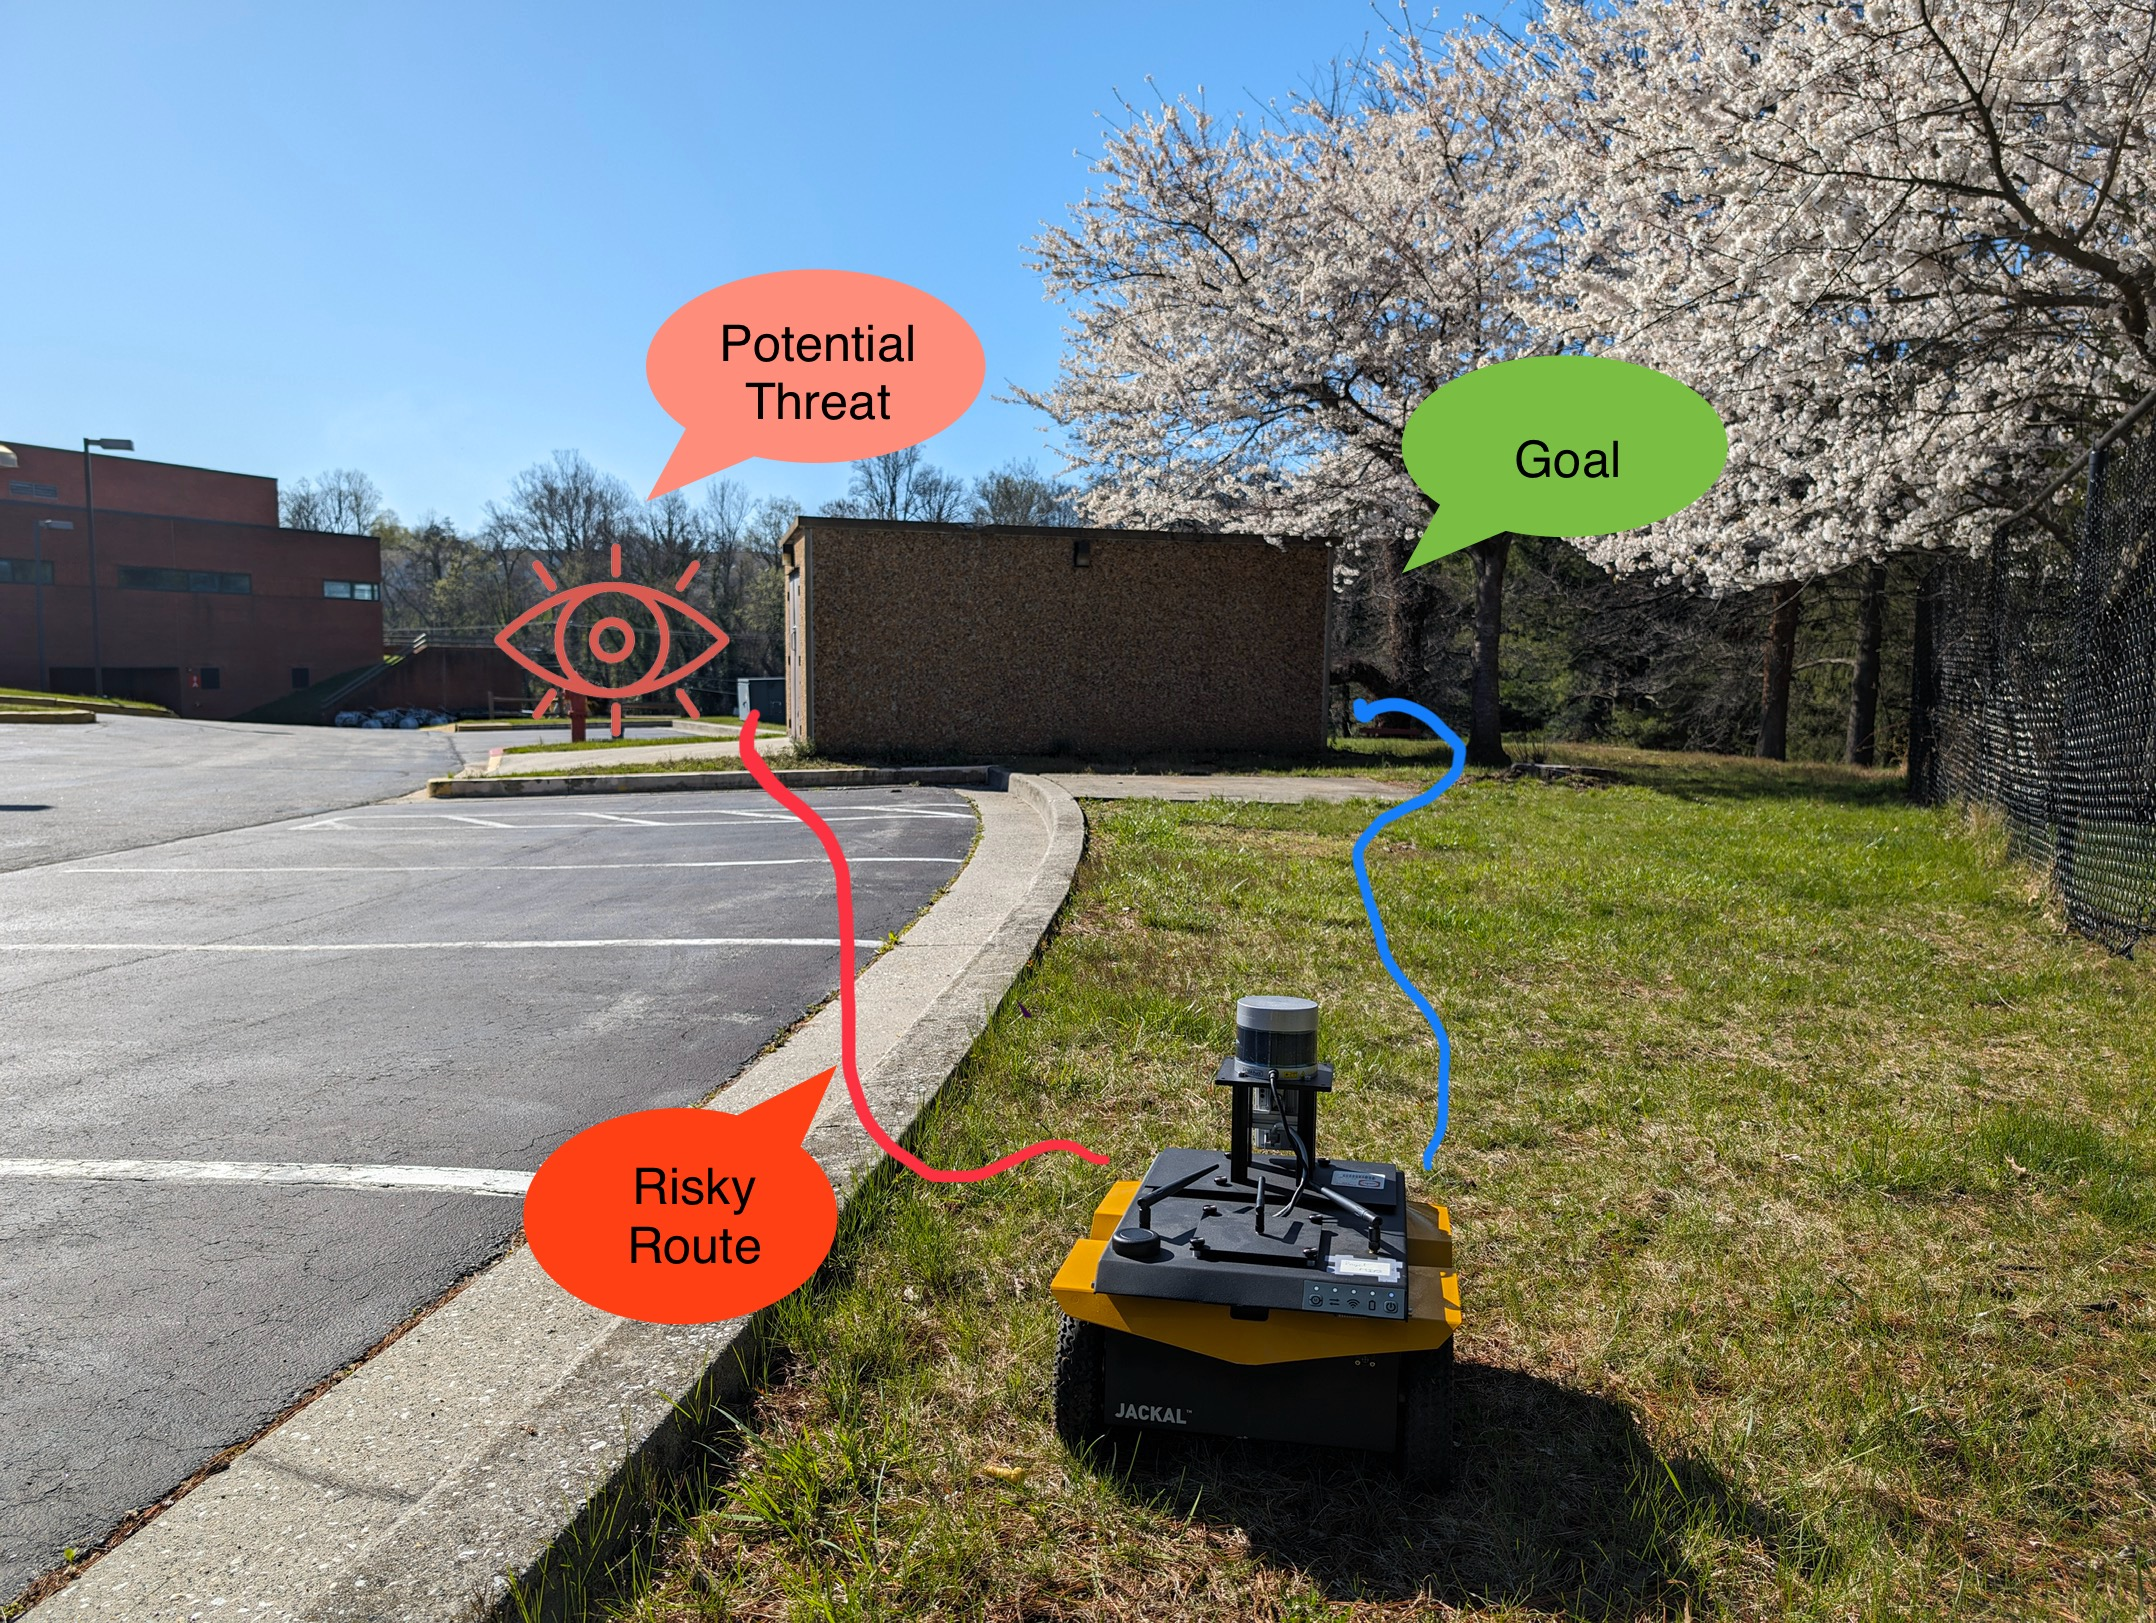
\includegraphics[width=\linewidth]{sections/images/covert_planning_2.jpeg}
    \caption{
    \textit{EnCoMP Covert Navigation Strategies}: 
In this outdoor environment, the robot (Jackal) is navigating towards a goal location. To achieve this while minimizing the risk of detection or interference from potential threats—defined as any external factors capable of recognizing or interfering with the robot's presence and objectives (represented by the eye icons)—the robot identifies and strategically moves toward nearby trees and a small brick building structure that can provide cover and concealment, instead of taking the risky route through the open area. By utilizing these natural and artificial features in the environment, the robot reduces its visibility and exposure as it traverses the field to reach its destination safely.}
   \label{fig}
\end{figure}

Reinforcement learning (RL) is a promising approach for autonomous navigation, enabling robots to learn complex strategies through interaction with the environment ~\cite{rl1, rl2}. Online RL methods have been applied to outdoor navigation ~\cite{online1, online2}, eliminating the need for human labeling. However, sim-to-real transfer issues ~\cite{sim2real1, sim2real2, weerakoon2022sim} often lead to severe performance degradation during real-world deployment of models trained using online reinforcement learning. In general, training complex models using online RL requires high-fidelity simulations, which may not be available for intricate environments. The discrepancies between the simulated and real-world domains can result in suboptimal performance when the trained models are applied to real-world scenarios. Offline RL ~\cite{offline1, offline2} has been proposed to mitigate these limitations by training models using data collected in real-world environments, reducing sim-to-real transfer problems. Despite the advancements in RL-based navigation, most existing methods have not fully exploited the rich information provided by modern sensors, such as LiDAR, which can offer valuable insights into the environment's properties and potential cover ~\cite{lidar1, lidar2}. 


To address these challenges, we propose an enhanced covert navigation framework that leverages LiDAR data, height maps, cover maps, potential threat maps, and offline reinforcement learning. Our approach enables robots to identify and utilize natural and artificial environmental features as cover, thereby minimizing exposure to potential threats while maintaining efficient navigation.


The main contributions of our work are as follows:

\begin{itemize}
  \item \textbf{Novel Offline Reinforcement Learning Framework for Covert Navigation:}
  We propose a novel offline reinforcement learning-based framework, \textit{EnCoMP}, to learn a Q-function that evaluates a ground robot's candidate actions in terms of their ability to maximize cover utilization, minimize threat exposure, and reach the goal efficiently in complex environments. The framework incorporates a state-of-the-art Conservative Q-Learning (CQL) model ~\cite{kumar2020conservative} that leverages LiDAR-based perception to capture rich environmental information. Our model is trained using a diverse real-world dataset collected in various environments, which is automatically processed to generate states, actions, and rewards. This offline learning approach mitigates the sim-to-real transfer issues present in existing reinforcement learning methods for covert robot navigation. \textit{EnCoMP} demonstrates a significant improvement of up to 20\% in terms of navigation success rate compared to existing approaches.

  \item \textbf{Mapping for Strategic Navigation Decision-Making:}
   We design an observation space that captures rich environmental information to facilitate intelligent decision-making. We introduce a novel combination of robot-centric height maps, cover maps, and threat maps generated from high-resolution LiDAR point cloud data. These maps provide detailed representations of terrain elevation, cover object presence and quality, and potential threat positions and line-of-sight, enabling the robot to assess traversability, strategically utilize cover, and proactively avoid threats. Additionally, we incorporate a goal map that encodes the relative distance and direction to the target location, guiding efficient navigation. This novel integration of LiDAR-based observations empowers \textit{EnCoMP} to make informed decisions prioritizing covert operation and goal-reaching.

  \item \textbf{Adaptive Threat-Aware Visibility Estimation (ATAVE) Algorithm:}
We introduce a dynamic probabilistic threat modeling technique, Adaptive Threat-Aware Visibility Estimation (ATAVE) Algorithm. This algorithm adapts in real-time to changes in the robot's sensory observations, providing a continuously updated assessment of potential environmental threats. ATAVE incorporates advanced visibility computation methods, including efficient line-of-sight checks and a prioritized tree structure for rapid threat evaluation. This allows for enhanced situational awareness and significantly improves decision-making under uncertain and dynamic conditions.

 \item \textbf{Performance Improvement:}
  We evaluate \textit{EnCoMP} in three different real-world outdoor covert navigation scenarios, including urban, forested, and mixed terrains. We measure the success rate, cover utilization, and threat exposure. We also compare the results with our previous work, CoverNav, which serves as a baseline. \textit{EnCoMP} achieves a 20\% improvement in average success rate, 25\% improvement in average cover utilization, and 15\% reduction in average threat exposure across the three covert navigation scenarios.
\end{itemize}

\vspace{1mm}

The remainder of this paper is organized as follows: Section \ref{related_work} provides an overview of related work in outdoor navigation. Some related background information is present in Section \ref{background} Section \ref{encomp_approach} presents our proposed covert navigation framework, detailing the perception pipeline, offline reinforcement learning algorithm, and policy transfer to a physical robot platform. Section \ref{sec:experiments} describes the experimental setup and presents the results of our real-world tests. Finally, Section \ref{conclusion} concludes the paper and discusses potential future research directions.